\documentclass{beamer}
%
% Choose how your presentation looks.
%
% For more themes, color themes and font themes, see:
% http://deic.uab.es/~iblanes/beamer_gallery/index_by_theme.html
%
\mode<presentation>
{
  \usetheme{Boadilla}      % or try Darmstadt, Madrid, Warsaw, ...
  \usecolortheme{beaver} % or try albatross, beaver, crane, ...
  \usefonttheme{default}  % or try serif, structurebold, ...
  \setbeamertemplate{navigation symbols}{}
  \setbeamertemplate{caption}[numbered]
  
} 

\usepackage{xcolor,colortbl}
\usepackage[english]{babel}
\usepackage[utf8x]{inputenc}
\usepackage{courier}
\usepackage{dsfont}
\usepackage{verbatim} 
\usepackage{enumerate}
\usepackage{tikz}
\usepackage{multirow}
\usepackage{bbm}
\usepackage{venndiagram}
\usepackage{epigraph} 
%\usepackage{xcolor}

%\usepackage{enumitem}

\usepackage{hyperref}
\hypersetup{
    colorlinks=true,
    linkcolor=blue,
    filecolor=magenta,      
    urlcolor=cyan,
}

% R stuff!
\usepackage{listings}
\definecolor{codegreen}{rgb}{0,0.6,0}
\definecolor{codegray}{rgb}{0.5,0.5,0.5}
\definecolor{codepurple}{rgb}{0.58,0,0.82}
\definecolor{backcolour}{rgb}{0.95,0.95,0.92}

\lstdefinestyle{mystyle}{
    backgroundcolor=\color{backcolour},    
    commentstyle=\color{codegreen},
    keywordstyle=\color{black},
    numberstyle=\tiny\color{codegray},
    stringstyle=\color{codepurple},
    basicstyle=\ttfamily\footnotesize,
    breakatwhitespace=false,         
    breaklines=true,                 
    captionpos=b,                    
    keepspaces=true,                 
    numbers=left,                    
    numbersep=5pt,                  
    showspaces=false,                
    showstringspaces=false,
    showtabs=false,                  
    tabsize=2
}

\lstset{style=mystyle}


\setbeamertemplate{enumerate items}[default]
\setbeamertemplate{itemize item}[triangle]

%\setitemize{label=\usebeamerfont*{itemize item}%
%  \usebeamercolor[fg]{itemize item}
%  \usebeamertemplate{itemize item}}



\title[SST-115 / STA-209]{Linear Regression -- Categorical Predictors}
\subtitle{}
\author{Grinnell College}
\date{September 27, 2024}

\graphicspath{{img/}}

\begin{document}

\begin{frame}
  \titlepage
\end{frame}

\begin{frame}{Review}

\begin{align*}
\hat{y}= b_0 +  b_1X
\end{align*}
On Wednesday, we spent some time talking about linear regression. Basically a fancy way of putting a line on a scatterplot to describe the relationship between variables.
\vspace{4mm}

\begin{itemize}
\item Only works when there is a \textit{linear} relationship
\item There are formulas for slope and intercept (use R!)
\item Use line to make predictions
\item Interpret the slope and intercept (if applicable)
\item $R^2$ and r
\end{itemize}
\end{frame}

%\begin{frame}{Today}
%What does it mean to use regression with a categorical predictor?
%\end{frame}



\begin{frame}{Review}
(`mpg` dataset)

Highway miles per gallon vs. City miles per gallon for vehicles 
\begin{center}
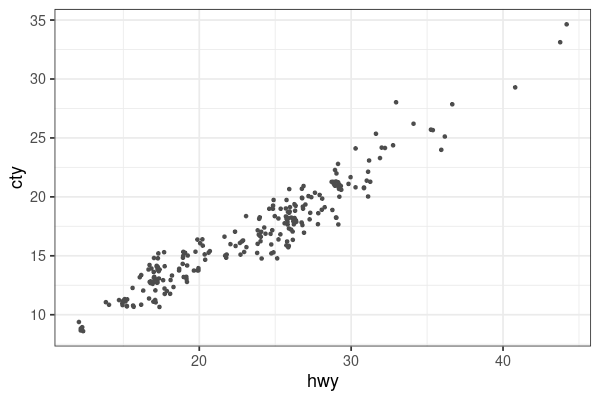
\includegraphics[scale=0.5]{reg_reg1.png}
\end{center}
\end{frame}


\begin{frame}
\begin{align*}
\widehat{\text{City mpg}}  = 0.844 + 0.683 \times \text{Highway mpg}
\end{align*}
\begin{center}
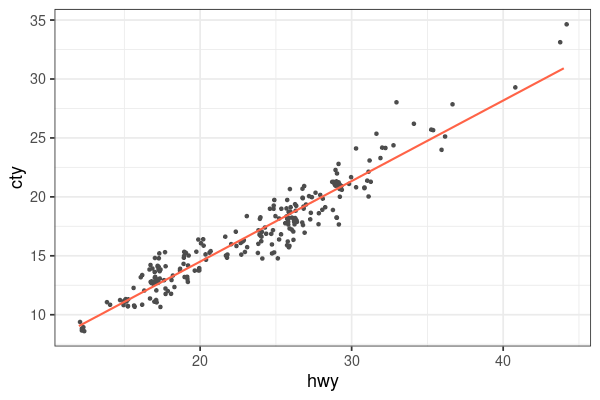
\includegraphics[scale=0.5]{reg_reg2.png}
\end{center}
\end{frame}



\begin{frame}{Categorical predictor?}
What if my explanatory variable was categorical? Can we use linear regression?
\begin{align*}
\hat{y} = \dots
\end{align*}
\begin{center}
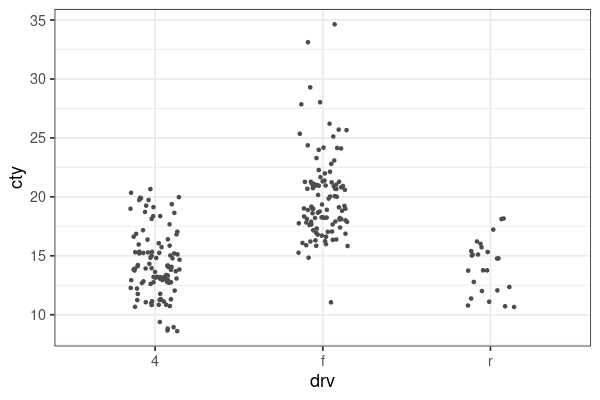
\includegraphics[scale=0.45]{cat_reg1.png}
\end{center}
\end{frame}


%\begin{frame}
%\begin{center}
%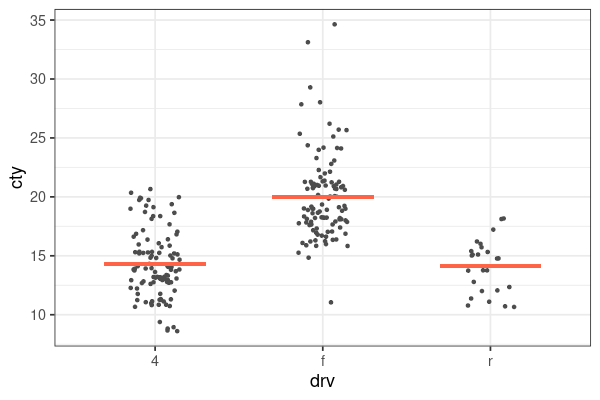
\includegraphics[scale=0.5]{cat_reg2.png}
%\end{center}
%\end{frame}

\begin{frame}{Indicator Variables}
Consider how data is stored in our data frames in R \vspace{4mm}
\begin{table}[ht]
\centering
\begin{tabular}{ll}
  \hline
Model & Transmission \\ 
  \hline
audi a4 & auto \\ 
  audi a4 & manual \\ 
  chevrolet c1500 suburban 2wd & auto \\ 
  dodge dakota pickup 4wd & auto \\ 
  ford explorer 4wd & manual \\ 
  hyundai sonata & auto \\ 
   \hline
\end{tabular}
\end{table}
\vspace{4mm}
How might these be used in regression?
\begin{itemize}
    \item force Transmission variable to be quantitative?
\end{itemize}
\end{frame}

\begin{frame}{Indicator Variables}
\textbf{Indicator Variables}: are a new variable we make that \textbf{indicates} whether an observation belongs to a specific category or not
\begin{itemize}
    \item sometimes called 'Dummy variables'
    \item 1 indicates an observation is in the category
    \item 0 indicates an observation is \textbf{not} in the category
\end{itemize}
\small
\begin{columns}
\begin{column}{0.45\textwidth}
\vspace{3mm}
\begin{table}[ht]
\centering
\begin{tabular}{ll}
  \hline
Model & Trans \\ 
  \hline
audi a4 & auto \\ 
  audi a4 & manual \\ 
  chevrolet c1500 & auto \\ 
  dodge pickup 4wd & auto \\ 
  ford explorer 4wd & manual \\ 
  hyundai sonata & auto \\ 
   \hline
\end{tabular}
\end{table}
\end{column}
\begin{column}{0.45\textwidth}  %%<--- here
\begin{table}[ht]
\centering
\begin{tabular}{lrr}
  \hline
Model & Manual & Auto \\ 
  \hline
audi a4 & 0 & 1 \\ 
  audi a4 & 1 & 0 \\ 
  chevrolet c1500  & 0 & 1 \\ 
  dodge pickup 4wd & 0 & 1 \\ 
  ford explorer 4wd & 1 & 0 \\ 
  hyundai sonata & 0 & 1 \\ 
   \hline
\end{tabular}
\end{table}
\end{column}
\end{columns}
\end{frame}


\begin{frame}{Indicator Variables}
\textbf{Indicator Variables} are often denoted with a stylistic "1" and a subscript to denote the original variable name \vspace{6mm}
\scriptsize
\begin{columns}
\begin{column}{0.45\textwidth}
\begin{table}[ht]
\centering
\begin{tabular}{lrr}
  \hline
Model & Manual & Auto \\ 
  \hline
audi a4 & 0 & 1 \\ 
  audi a4 & 1 & 0 \\ 
  chevrolet c1500  & 0 & 1 \\ 
  dodge pickup 4wd & 0 & 1 \\ 
  ford explorer 4wd & 1 & 0 \\ 
  hyundai sonata & 0 & 1 \\ 
   \hline
\end{tabular}
\end{table}
\end{column}
\begin{column}{0.45\textwidth}  %%<--- here
\begin{align*}
\mathbbm{1}_{\text{Manual}} = \begin{cases}
1 \quad \text{if Manual}\\ 
0 \quad \text{if Automatic}
\end{cases}
\end{align*}
\begin{align*}
\mathbbm{1}_{\text{Automatic}} = \begin{cases}
1 \quad \text{if Automatic}\\ 
0 \quad \text{if Manual}
\end{cases}
\end{align*}
\end{column}
\end{columns}
\end{frame}


\begin{frame}{Indicator Variables}
Maybe we can make predictions for groups using their averages?
\scriptsize
\begin{columns}
  \begin{column}{0.45\textwidth}
	\begin{center}
	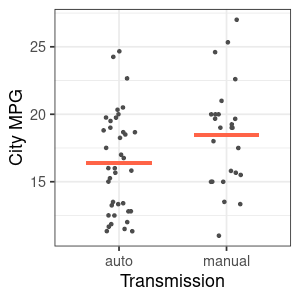
\includegraphics[scale=0.5]{trans_reg.png}
	\end{center}
  \end{column}

  \begin{column}{0.5\textwidth}
% latex table generated in R 4.4.1 by xtable 1.8-4 package
% Sun Sep 22 11:51:26 2024
\begin{table}[ht]
\centering
\begin{tabular}{lrrr}
  \hline
Model & Manual & Auto & cty \\ 
  \hline
audi a4 & 0 & 1 & 18.250 \\ 
  audi a4 & 1 & 0 & 19.667 \\ 
  chevy c1500 & 0 & 1 & 12.800 \\ 
  dodge pickup & 0 & 1 & 12.500 \\ 
  ford explorer & 1 & 0 & 15.000 \\ 
  hyundai sonata & 0 & 1 & 19.000 \\ 
   \hline
\end{tabular}
\end{table}

\begin{table}[ht]
\centering
\begin{tabular}{lr}
  \hline
Transmission & Average City MPG \\ 
  \hline
auto & 16.370 \\ 
  manual & 18.457 \\ 
   \hline
\end{tabular}
\end{table}
  \end{column}
\end{columns}

\begin{align*}
\widehat{\text{City mpg}} = 16.370 \times \mathbbm{1}_{\text{Automatic}} + 18.457 \times \mathbbm{1}_{\text{Manual}}
\end{align*}
\end{frame}

\begin{frame}[fragile]{Linear Model in R}
\small
By default, the first indicator will be absorbed into the intercept, making it the \textit{reference variable}
\begin{lstlisting}[language=R]
> lm(cty ~ trans, mpg2)

Coefficients:
(Intercept)  transmanual  
      16.37         2.09  
\end{lstlisting}

Compare equations:

\begin{align*}
\widehat{\text{City mpg}} &= 16.37 \times \mathbbm{1}_{\text{Automatic}} + 18.457 \times \mathbbm{1}_{\text{Manual}} \\
\widehat{\text{City mpg}} &= 16.37 + 2.09 \times \mathbbm{1}_{\text{Manual}}
\end{align*}
\end{frame}


\begin{frame}{Practice}
\scriptsize
More than 2 categories?!

What are my indicator variables going to look like?

\begin{columns}
\begin{column}{0.45\textwidth}
\vspace{3mm}
% latex table generated in R 4.3.2 by xtable 1.8-4 package
% Fri Feb 16 09:57:05 2024
\begin{table}[ht]
\centering
\begin{tabular}{lrl}
  \hline
model & cty & drv \\ 
  \hline
new beetle &  21 & f \\ 
  gti &  19 & f \\ 
  mustang &  18 & r \\ 
  grand cherokee 4wd &  11 & 4 \\ 
  sonata &  21 & f \\ 
  civic &  24 & f \\ 
  toyota tacoma 4wd &  15 & 4 \\ 
   \hline
\end{tabular}
\end{table}
\end{column}
\begin{column}{0.45\textwidth}  %%<--- here

\end{column}
\end{columns}

Categories of `drv`: 4-wheel drive (4), rear-wheel drive (r), front-wheel drive (f)
\end{frame}


\begin{frame}{Practice}
\scriptsize
Categories of `drv`: 4-wheel drive (4), rear-wheel drive (r), front-wheel drive (f) \vspace{3mm}

What are my indicator variables going to look like?
\begin{columns}
\begin{column}{0.3\textwidth}
% latex table generated in R 4.3.2 by xtable 1.8-4 package
% Fri Feb 16 09:57:05 2024
\begin{table}[ht]
\centering
\begin{tabular}{lrl}
  \hline
model & cty & drv \\ 
  \hline
new beetle &  21 & f \\ 
  gti &  19 & f \\ 
  mustang &  18 & r \\ 
  grand cherokee &  11 & 4 \\ 
  sonata &  21 & f \\ 
  civic &  24 & f \\ 
  toyota tacoma &  15 & 4 \\ 
   \hline
\end{tabular}
\end{table}
\end{column}
\begin{column}{0.5\textwidth}  %%<--- here
\vspace{3mm}
% latex table generated in R 4.3.2 by xtable 1.8-4 package
% Fri Feb 16 10:01:11 2024
\begin{table}[ht]
\centering
\begin{tabular}{lrrrr}
  \hline
model & cty & drvf & drvr & drv4 \\ 
  \hline
new beetle & 21 & 1 & 0 & 0 \\ 
  gti & 19 & 1 & 0 & 0 \\ 
  mustang & 18 & 0 & 1 & 0 \\ 
  grand cherokee & 11 & 0 & 0 & 1 \\ 
  sonata & 21 & 1 & 0 & 0 \\ 
  civic & 24 & 1 & 0 & 0 \\ 
  toyota tacoma & 15 & 0 & 0 & 1 \\ 
   \hline
\end{tabular}
\end{table}
\end{column}
\end{columns}
\end{frame}




\begin{frame}[fragile]{Practice}
\footnotesize
Categories of `drv`: 4-wheel drive (4), rear-wheel drive (r), front-wheel drive (f)
\begin{lstlisting}[language=R]
> lm(cty ~ drv, mpg)

Coefficients:
(Intercept)         drvf         drvr  
      14.33         5.64        -0.25  
\end{lstlisting}

\begin{itemize}
\item What is the \textit{reference variable}
\item Equation for line?
\item Interpretation of intercept? Slope?
\item What is the average city mileage for:
\begin{itemize}\footnotesize
	\item 4-wheel drive?
	\item Front-wheel drive?
	\item Rear-wheel drive?
\end{itemize}
\end{itemize}

\end{frame}



\begin{frame}[fragile]{Practice}
\footnotesize
\begin{lstlisting}[language=R]
> lm(cty ~ drv, mpg)

Coefficients:
(Intercept)         drvf         drvr  
      14.33         5.64        -0.25  
\end{lstlisting}

\begin{center}
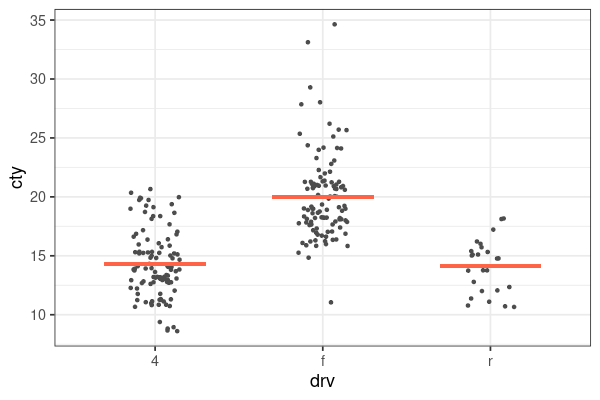
\includegraphics[scale=0.4]{cat_reg2.png}
\end{center}
\end{frame}

\begin{frame}[fragile]{Extending to Multiple Variables}

Here we have the average city miles per gallon for each combination of drive train and transmission



\begin{columns}

  \begin{column}{0.45\textwidth}
  {\footnotesize
\begin{table}[ht]
\centering
\begin{tabular}{lrrr}
  \hline
Transmission & 4wd & fwd & rwd \\ 
  \hline
Automatic &  13.85 & 19.11 & 13.29 \\
Manual & 15.61 & 21.34 & 15.75 \\  \hline
\end{tabular}
\end{table}
}
  \end{column}
  \begin{column}{0.45\textwidth}
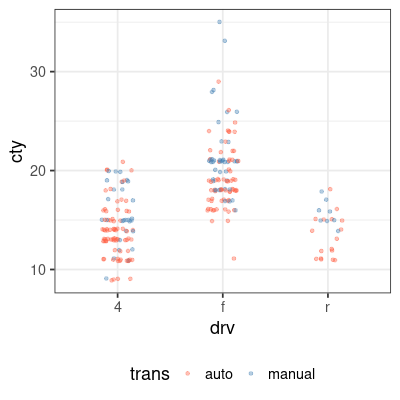
\includegraphics[scale=.4]{double_cat_pred1.png}
  \end{column}

\end{columns}

\end{frame}

\begin{frame}[fragile]{Extending to Multiple Variables}

\begin{lstlisting}[language=R]
> lm(cty ~ drv + trans, mpg)

Coefficients:
(Intercept)         drvf         drvr  transmanual  
      13.77         5.40        -0.35         2.07 
\end{lstlisting}


\begin{itemize}
\item What is the \textit{reference variable}
\item Equation for line?
\item Interpretation of intercept? Slope?
\item What is the average city mileage for:
\begin{itemize}\footnotesize
	\item Automatic 4-wheel drive?
	\item Manual Front-wheel drive?
\end{itemize}
\end{itemize}

\end{frame}

\begin{frame}[fragile]{Observed vs Predicted Means}
\begin{lstlisting}[language=R]
> lm(cty ~ drv + trans, mpg)

Coefficients:
(Intercept)         drvf         drvr  transmanual  
      13.77         5.40        -0.35         2.07 
\end{lstlisting}

Observed: \\
\begin{table}[ht]
\centering
\begin{tabular}{lrrr}
  \hline
Transmission & 4wd & fwd & rwd \\ 
  \hline
Automatic &  13.85 & 19.11 & 13.29 \\
Manual & 15.61 & 21.34 & 15.75 \\  \hline
\end{tabular}
\end{table}

Predicted: \\

\begin{table}[ht]
\centering
\begin{tabular}{lrrr}
  \hline
Transmission & 4wd & fwd & rwd \\ 
  \hline
Automatic &  13.76 & 19.17 & 13.42 \\
Manual & 15.83 & 21.24 & 15.49 \\  \hline
\end{tabular}
\end{table}

\end{frame}

\begin{frame}
\begin{center}
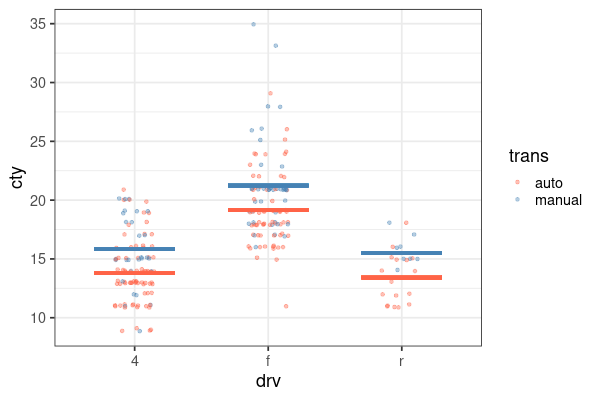
\includegraphics[scale=0.5]{double_cat_pred.png}
\end{center}
\end{frame}


%
%
%\begin{frame}{Regression with Categorical Predictors}
%Predict enrollment from private or public \\
%
%indicator variables
%
%bonus intercepts not slopes
%\end{frame}
%
%\begin{frame}
%another example looking at enrollment by region, what is reference var, see it's like conditional mean, i.e., given x here is y except one continuous and one discrete
%\end{frame}
%

%%%%%%%%%%%%%%%%

%\begin{frame}
%\begin{columns}
%
%  \begin{column}{0.45\textwidth}
%%
%  \end{column}
%  \begin{column}{0.45\textwidth}
%%
%  \end{column}
%
%\end{columns}
%\end{frame}


\end{document}